\chapter{Privacy}\label{privacy}

Uno degli obiettivi del design di Bitcoin è l'anonimato dell'utente. Il paragone più appropriato è quello con i conti in banca della Svizzera. Ogni utente bitcoin può infatti possedere più di un portafogli (ovvero di una coppia di chiavi pubblica e privata) e per ogni portafogli più di un conto/indirizzo (che altro non è che una stringa unica generata grazia alla coppia di chiavi) e tutte le transazioni si basano unicamente sull'indirizzo. Non esiste quindi nessun modo per risalire al proprietario di un dato indirizzo bitcoin basandosi unicamente sulla struttura della rete.

Esistono ovviamente diverse tecniche sia per ridurre il livello di privacy, ad esempio tramite il furto delle chiavi o un'analisi statistica degli input e degli output delle transazioni, sia per aumentarlo, magari creando un diverso portafoglio per ogni conto che si desidera creare.

\section{Analisi quantitativa della privacy}\label{analisi-quantitativa-della-privacy}

Ma come si fa a misurare il livello di privacy offerto da Bitcoin? In questa sezione si discuteranno alcune metriche arbitrarie create appositamente che trattano i vari aspetti dell'anonimato nella rete Bitcoin.

Essendo una analisi quantitativa, è necessario fornire una definizione formale per i termini fin qui usati in modo più o meno descrittivo. Sotto tale ottica verrano quindi proposte alcune definizioni formali, la prima delle quali è il concetto portante della rete:

Transazione:
\[\tau(a_{\textrm{S}} \rightarrow a_{\textrm{R}}) = \{ \textrm{source}, B, a_{\textrm{R}}, \textrm{SIG}_{\textrm{sk}_{a_{\textrm{S}}}}\left(\textrm{source}, B, a_{\textrm{R}}\right) \} \]
definisce una transazione che intercorre tra i due indirizzi $a_{\textrm{S}}$ e $a_{\textrm{R}}$, in cui $\textrm{SIG}_{\textrm{sk}_{a_{\textrm{S}}}}$ è la firma digitale creata utilizzando la chiave privata $\textrm{sk}_{a_\textrm{S}}$ corrispondente alla chiave pubblica associata all'indirizzo $a_\textrm{S}$. $B$ è la quantità di BTC trasferite e $\textrm{source}$ è un riferimento alla più recente transazione da cui $a_\textrm{S}$ ha ottenuto le $B$ BTC.

Al fine dell'analisi, assumiamo la situazione tipica della rete Bitcoin, in cui ogni singolo utente dispone di diversi indirizzi a lui associati. Mentre questa può sembrare una forzatura, in realtà non lo è affatto. Come abbiamo detto in precedenza, ogni transazione contiene un indirizzo di ritorno per il resto. Tale indirizzo viene definito \emph{indirizzo ombra} ed è creato automaticamte senza l'intervento dell'utente. Per cui ogni utente possiede almeno due indirizzi: quello creato al momento della creazione del portafogli e l'indirizzo ombra.

\subsection{Il modello antagonistico}\label{il-modello-antagonistico}

Gli algoritmi proposti consistono nell'osservazione del log pubblico di Bitcoin (\emph{pubLog}) durante un periodo $\Delta t$. Durante questo periodo, $n_U $ utenti (dall'insieme $U = \{u_1, \ldots, u_{n_U}\}$) contribuiscono al \emph{pubLog} con l'insieme di indirizzi $A = \{a_1, \ldots, a_{n_A}\}$. Si ha poi l'insieme delle transazioni $T = \{ \tau_1 (S_1 \rightarrow R_1), \ldots , \tau_{n_T}(S_{n_T} \rightarrow R_{n_T}) \} $ in cui $\tau_i (S_i \rightarrow R_i)$ descrive una singola transazione con ID univoco pari a $i$, e con $S_i$ e $R_i$ l'insieme degli indirizzi di mittente e destinatario rispettivamente. Viene introdotto anche un avversario $\adversary$ interessato ad ottenere informazioni su tutte le transazioni e gli indirizzi appartenenti ad un insieme di utenti Bitcoin. Si assume quindi che $\adversary$ sia un nodo legittimo della rete, abbia accesso a \emph{pubLog}, ad alcuni indirizzi di commercianti resi pubblici e altre informazioni statistiche pubblicamente disponibili. Inoltre si assume anche che gli utenti siano incoraggiati a cambiare frequentemente i loro indirizzi, spostando le loro monete da un indirizzo all'altro. Questa è una delle abitudini consigliate da Nakamoto.

\subsection{Quantificazione della Privacy}\label{quantificazione-della-privacy}

Esistono (almeno) due nozioni distinte di privacy per la rete Bitcoin.

\emph{Activity unlinkability}: Un avversario $\adversary$ non dovrebbe essere in grado di associare due indirizzi distinti (\emph{address unlinkability}) o transazioni (\emph{transaction unlinkability}) ad un utente scelto dell'avversario stesso.

\emph{Profile indistinguishability}: L'avversario non deve essere in grado di ricostruire i profili (insieme di indirizzi e transazioni) di tutti gli utenti del \emph{pubLog}. Questa nozione di privacy è più forte della precedente, in quanto riguarda l'intera rete e non solo un utente. Inoltre i due profili (per transazioni e per indirizzi) non sono equivalenti quando si tratta di modellare il profilo di un utente, in quanto è possibile indovinare correttamente gli indirizzi di utenti coinvolti in poche transazioni ma sbagliare nel caso di pochi indirizzi coinvolti in molte transazioni.

Vengono definiti due algoritmi \emph{AddUnl} e \emph{ProfInd} che implementano una sorta di sfida in cui l'attaccante tenta di violare le due nozioni di privacy sopra descritte. Il risultato sarà una quantificazione delle nozioni di privacy nei termini del vantaggio che $\adversary$ possiede per vincere queste sfide nei confronti di un avversario $\adversaryrnd$ che tenta di vincere le stesse sfide rispondendo in modo casuale. Ipotizziamo che $\adversary$ abbia accesso completo a \emph{pubLog} e che sia $\adversary$ che $\adversaryrnd$ abbiano accesso ad una base di conoscenza comune $\knowa$ che contengono informazioni verificate su un sottoinsieme di indirizzi e i relativi proprietari.

\subsubsection{Address Unlinkability}\label{address-unlinkability}

Il seguente algoritmo descrive il meccanismo con cui avviene la sfida per la address unlinkability. In questo algoritmo si utilizza $\adversary$ come un generico avversario, in quanto per i calcoli di quantificazione l'algoritmo verrà eseguito sia da $\adversary$ che da $\adversaryrnd$. Si comincia con $\adversary$ che seleziona in modo causale un indirizzo presente in pubLog e lo invia ad uno sfidante $\challenger$ (che si assume sia a conoscenza delle corrette correlazioni utenti-indirizzi). Se l'indirizzo scelto da $\adversary$ è l'unico che appartiene all'utente, $\adversary$ vince la sfida. Altrimenti $\challenger$ scegli un bit casuale $\mathit{b}$. Se $\mathit{b} = 1$ allora $\challenger$ sceglie un nuovo indirizzo tra quelli disponibili in pubLog che appartenga allo stesso utente del primo indirizzo, altrimenti il nuovo indirizzo verrà scelto tra quelli in pubLog che non appartengono al proprietario del nuovo indirizzo. L'indirizzo scelto insieme al precedente indirizzo vengono inviati ad $\adversary$, il quale stima (con un algoritmo di sua scelta, ininfluente per la sfida) se i due indirizzi che ha ricevuto appartengono o meno allo stesso utente, e memorizza il suo risultato nel bit $\mathit{b}'$. Se $\adversary$ ha indovinato, ovvero se $\mathit{b} = \mathit{b}'$, allora $\adversary$ vince la sfida. L'algoritmo è visibile in \ref{addunl_alg}.

\begin{algorithm}
	\caption{Address Unlinkability}
	\label{addunl_alg}
	\begin{algorithmic}
		AddUnl(A, \challenger, \knowa$, pubLog):
		\STATE $a_0 \leftarrow $A.randomAddr(pubLog)
		A.send($a_0, \challenger$)
		\IF{$\challenger$.isUniqueAddr($a_0$)
			A.win()
		\ELSE
			$\mathcol{b} \leftarrow \challenger$.randomBit()
			\IF{$\mathcol{b} = 1$}
				$a_1 \leftarrow \challenger$.sameUsrAddr($a_0$, pubLog)
			\ELSE
				$a_1 \leftarrow \challenger$.otherUsrAddr($a_0$, pubLog)
			\ENDIF
			$\challenger$.send($\langle a_0, a_1 \rangle$, A)
			$\mathcol{b}' \leftarrow $A.estimateSameUser($a_0, a_1$)
			\IF{$\mathcol{b} = \mathcol{b}'$} A.win() \ENDIF
		\ENDIF
	\end{algorithmic}
\end{algorithm}


Stabiliamo che Bitcoin soddisfa il principio di \emph{Address Unlinkability} se, per ogni avversario $\adversary$ (che ha un ben preciso algoritmo per rispondere alla domanda di $\challenger$) e per ogni coppia di indirizzi scelti dall'algoritmo, $\adversary$ ha solo un piccolo vantaggio rispetto ad un avversario come $\adversaryrnd$ che risponde a caso alla domanda posta da $\challenger$. Formalmente diciamo che Bitcoin soddisfa la Address Unlinkability se:

\begin{equation*}
\Pr [ \mathit{b}' \leftarrow \adversary \left(\text{pubLog}, \knowa \right) : \mathit{b} = \mathit{b}' ] - \Pr [\mathit{b}' \leftarrow \adversaryrnd \left(\knowa \right) : \mathit{b} = \mathit{b}' ] \leq \varepsilon
\end{equation*}

con $\varepsilon$ trascurabile.

\paragraph{Quantificazione di Address Unlinkability}\label{quantificazione-di-address-unlinkability}

Sfruttando i risultati ottenuti dalla sfida, è possibile stimare il \emph{grado} con cui gli indirizzi Bitcoin possono essere collegati ad uno stesso utente. Verranno definite alcune strutture matematiche necessarie per i calcoli.

\[E_\text{link} [i, j] = \{p_{i,j}\}_{i,j \in [1, n_A ]}\]

Rappresenta una matrice $n_A \times n_A$ in cui ogni argomento esprime la probabilità $p_{i,j}$ stimata da $\adversary$ che l'indirizzo $a_i$ appartenga allo stesso utente dell'indirizzo $a_j$ (in simboli, $a_i \sameuser a_j$). Si definisce poi una matrice $n_A \times n_A$ che mantenga le informazioni sulle reali connessioni tra gli indirizzi:

\[\text{GT}_\text{link} [i,j] = \begin{cases} 1 &\text{se } a_i \sameuser a_j \\ 0 &\text{altrimenti} \end{cases}\]

Date queste due strutture, si definisce l'errore commesso da $\adversary$ nella sua stima come la \emph{distanza di Manhattan} che intercorre tra $E_\text{link} [i,*]$ e le vere associazioni di $a_i$ con tutti gli indirizzi in pubLog:

\[ \begin{aligned} \text{Er}_{\adversary} &= \| E_\text{link} [i, *] - \text{GT}_\text{link} [i,*]\|_1 \\
   &= \sum_x | E_\text{link} [i, x] - \text{GT}_\text{link} [i,x] | \quad \text{ con } x \in [1, n_A]
   \end{aligned}\]

Si può dunque determinare il successo di $\adversary$ per AddUnl come il massimo del suo errore:

\[ \begin{aligned} \text{Succ}_{\adversary} &= \max_{\forall a_i \not\in \knowa} \left(\| E_\text{link} [i, *] - \text{GT}_\text{link} [i,*]\|_1 \right) \\
   &= \max_{\forall a_i \not\in \knowa}\left(\sum_x | E_\text{link} [i, x] - \text{GT}_\text{link} [i,x] |\right) \quad \text{ con } x \in [1, n_A]
   \end{aligned} \]

Stesse condizioni devono essere fatte per l'avversario con criterio di decisione casuale, $\adversaryrnd$. Mantenendo uguale $\text{GT}_\text{link} [i,j]$ è necessario definire la matrice $E^{\mathcal{R}}$\_come segue:

\[E^{\mathcal{R}}_\text{link} [i, j] = \begin{cases} \pi_{i,j} &\text{ se } \langle a_i, a_j \rangle \in \knowa \\ \rho + \rho(1-\rho)\tfrac{1}{2} &\text{ altrimenti} \end{cases}\]

Dove $\pi_{i,j}$ rappresenta la probabilità che gli indirizzi $a_i$ e $a_j$ appartengano allo stesso utente secondo $\knowa$, mentre $\rho$ è la frazione di indirizzi in $\{\text{pubLog} \smallsetminus \knowa\}$ che non può essere associata ad altri indirizzi (il che capita quando un utente ha solo un indirizzo)\footnote{l'esistenza degli indirizzi ombra   non ha al momento rilevanza, ma più avanti $\rho$ diventerà   trascurabile a causa della loro presenza.}. Per le coppie di indirizzi non incluse in $\knowa$ tale probabilità è $\rho + \rho(1-\rho)\tfrac{1}{2}$.

Le altre formule vengono mantenute uguali sostituendo $E^{\mathcal{R}}_\text{link} [i, j]$ a $E_\text{link} [i, j]$. Il grado di address unlinkability risulta quindi essere il grado di successo aggiuntivo che $\adversary$ può ottenere da pubLog in comparazione con $\adversaryrnd$, chiamato $Link^{\text{abs}}_{\adversary}$
%FIXME   non ho la minima idea di cosa sia la versione normalizzata.

\[ \begin{aligned} Link^{\text{abs}}_{\adversary} &= \text{Succ}_{\adversary} - \text{Succ}_{\adversaryrnd} \\
   &= \frac{\text{Succ}_{\adversary} - \text{Succ}_{\adversaryrnd}}{\text{Succ}_{\adversaryrnd}} \quad \text{ in versione normalizzata}
   \end{aligned}\]

\subsubsection{User Profile Indistinguishability}\label{profile-indistinguishability}

L'impossibilità di ricostruire i profili di tutti gli utenti è una proprietà molto più forte rispetto all'impossibilità di associare due indirizzi diversi ad uno stesso utente.

L'algortimo di sfida \emph{ProfInd}\label{profind_alg} viene costruito nel modo seguente.
Lo sfidante $\challenger$ invia ad $\adversary$ il numero $n_U$ di utenti in $\{\text{pubLog} \smallsetminus \knowa\}$, che risponde con $n_U$ insiemi di indirizzi (o transazioni) e con la matrice $E_\text{prof} = {\{g_i\}}^{n_U}_{i=1}$ rappresentante la stima fatta da $\adversary$ sui profili degli utenti nel sistema.
Come per l'algoritmo precedente, definiamo $\text{GT}_\text{prof} = {\{\text{gt}_i\}}^{n_U}_{i=1}$ che rappresenta le vere associazioni tra indirizzi (o transazioni) e utenti, per cui:

\[
	\text{GT}_\text{prof} = \begin{cases}
		{\{a_{u_i}\}}^{n_U}_{i=1} &\text{ per profili basati su indirizzi} \\
		{\{\tau_{u_i}\}}^{n_U}_{i=1} &\text{ per profili basati su transazioni}
	\end{cases}
\]

dove $a_{u_i}$ e $\tau_{u_i}$ rappresentano insiemi di indirizzi/transazioni per l'utente $u_i$.
Ovviamente, $\adversary$ vince la sfida se indovina correttamente il profilo, ovvero $E_\text{prof} \equiv \text{GT}_\text{prof}$.

\begin{algorithm}
	\caption{ProfInd}
	\label{profind_alg}
	\begin{algorithmic}
		\STATE $\challenger$.send($n_U$, A)
		\STATE $E_\text{prof} \leftarrow$ A.estimateProfile()
		\IF{$E_\text{prof} = \text{GT}_\text{prof}$}
			\STATE A.win()
		\ENDIF
	\end{algorithmic}
\end{algorithm}


Diciamo che un sistema soddisfa la proprietà di \emph{Profile Indistinguishability} se non esiste nessun avversario $\adversary$ in grado di vincere \emph{ProfInd} con una probabilità migliore dell'avversario che risponde casualmente $\adversaryrnd$, ovvero:

\[
	\begin{aligned}
		\forall \adversary: &\Pr [E_\text{prof} \leftarrow \adversary(\text{pubLog}, n_U): E_\text{prof} \equiv \text{GT}_\text{prof}] - \\
		&\Pr [ E^\mathcal{R}_\text{prof} \leftarrow \adversaryrnd(n_U) : E^\mathcal{R}_\text{prof} \equiv \text{GT}_\text{prof} ] \leq \varepsilon
	\end{aligned}
\]

\paragraph{Quantificazione di Profile Indistinguishability}\label{quantificazione-di-profile-indistinguishability}

Anche in questa stima come per la precedente, la quantificazione dipende dal confronto tra la stima di $\adversary$ e i dati reali.
Definiamo quindi la similitudine tra $E_\text{prof}$ e $\text{GT}_\text{prof}$ come la funzione $Sim(E_\text{prof}, \text{GT}_\text{prof})$, i cui valori appartengono all'insieme $[0, 1]$.
Come per la address unlinkability, misuriano la profile indistinguishability contro $\adversary$ stimando il grado con cui $\adversary$ è in grado di stilare un profilo utente corretto, ovvero misurando il vantaggio che $\adversary$ ha rispetto a $\adversaryrnd$ nell'avvicinarsi a $\text{GT}_\text{prof}$:

\[ \text{Prof}_\adversary = \text{Sim}(E_\text{prof}, \text{GT}_\text{prof}) - \text{Sim}(E^\mathcal{R}_\text{prof}, \text{GT}_\text{prof}) \]

Per quantificare $Sim(E_\text{prof}, \text{GT}_\text{prof})$ e $\text{Prof}_\adversary$ è necessario sfruttare alcune metriche per calcolare le distanze basate sull'entropia, la \gls{nmi} e la \gls{ami}.
La \gls{nmi} valuta la similarità di due raggruppamenti degli stessi oggetti e assume valori tanto più alti (il massimo è 1) tanto più i due raggruppanti sono identici.
La \gls{ami}, dati due raggruppamenti $G_1$ e $G_2$, si avvicina allo 0 quando $G_1$ risulta simile ad un raggruppamento casuale, mentre si avvicina a 1 quando $G_1 = G_2$. Quindi \gls{ami} valuta direttamente il vantaggio che ha $\adversary$ nel vincere la sfida di \emph{ProfInd}.

Nel caso di profili basati sugli indirizzi, \gls{nmi} e \gls{ami} sono calcolate come segue:

\[\text{NMI} = \frac{\mathcal{I} \left(E_\text{prof}, \text{GT}_\text{prof}\right)}{\max \left(H \left(E_\text{prof}\right),H \left(\text{GT}_\text{prof}\right)\right)} \]
\[\text{AMI} = \frac{\mathcal{I} \left(E_\text{prof}, \text{GT}_\text{prof} - \mathcal{E}\right)}{\max \left(H \left(E_\text{prof}\right),H \left(\text{GT}_\text{prof}\right)\right) - \mathcal{E}}\]
dove:
\[ \mathcal{I} \left(E_\text{prof}, \text{GT}_\text{prof}\right) = \sum^{n_U}_{i=1} \left( \sum^{n_U}_{i=1} \left( \frac{n_{\left(i,j \right)}}{n_A} \log\left(\frac{n_{\left(i,j\right)} \cdot n_A}{n_{\left(i,*\right)}n_{\left(*,j\right)}}\right)\right)\right) \]
\[ H\left(E_\text{prof}\right) = - \sum^{n_U}_{i=1} \left(\frac{n_{\left(i,*\right)}}{n_A} \log\left(\frac{n_{\left(i,*\right)}}{n_A}\right)\right) \]
\[ H\left(\text{GT}_\text{prof}\right) = - \sum^{n_U}_{j=1} \left(\frac{n_{\left(*,j\right)}}{n_A} \log\left(\frac{n_{\left(*,j\right)}}{n_A}\right)\right) \]
\[
	\scriptstyle \mathcal{E} = \sum^{n_U}_{i=1} \left(
	    \sum^{n_U}_{j=1} \left(
	        \sum_{n \in \mathcal{M}} \left(
	            \frac{n}{n_A} \log \left(
	                \frac{n_A n}{n_{\left(i, *\right)} n_{\left(*, j \right)}}
	            \right) \frac{n_{\left(i, *\right)}! n_{\left(*, j\right)}! \left(
	                n_A - n_{\left(i, *\right)}
	            \right)!\left(
	                n_A - n_{\left(*, j\right)}
	            \right)!}
	            {n_A!\left(n_{\left(i, *\right)} - n\right)!
	                    \left(n_{\left(*, j\right)} - n\right)!
	                    \left(n_A - n_{\left(i, *\right)} - n_{\left(*, j\right)} - n \right)!}
	            \right)
	        \right)
	    \right)
\]
\[ \mathcal{M} = \left[ \max \left( n_{\left(i,*\right)} + n_{\left(*,j\right)} - n_A, 0\right), \min\left(n_{\left(i,*\right)}, n_{\left(*,j\right)}\right)\right] \]

%TODO tradurre "expected mutual information"
In queste formule, $n_A$ è il numero di indirizzi Bitcoin, $n_{\left(i,j\right)}$ è il numero di indirizzi di $u_i$, che vengono assegnati al gruppo $g_j$, $n_{\left(i,*\right)}$ e $n_{\left(*,j\right)}$ sono il numero di indirizzi di $u_i$ e $g_i$ rispettivamente. $\mathcal{E}$ rappresenta l'informazione mutuale attesa tra il raggruppamento $\text{GT}_\text{prof}$ e il raggruppamento casuale di indirizzi $E^\mathcal{R}_\text{prof}$.
Si possono ottenere risultati simili per calcolare \gls{nmi} e \gls{ami} nel caso di profili basati sulle transazioni.

È importante far presente che, sebbene \gls{nmi} e \gls{ami} siano efficaci per rappresentare il successo di $\adversary$ nella creazione di un profilo per tutti gli utenti della rete, non sono in grado di misurare il successo dell'avversario nel creare un profilo per un utente specifico.
Nella sezione \ref{risultati-simulazione} verrà misurato il successo di $\adversary$ nel creare il profilo di un utente specifico $u_i$ stabilendo la massima similitudine degli indirizzi (o transazioni) di $u_i$ con ogni cluster avversario, ovvero $ \max_{\forall j} = \left( \text{Sim}\left(a_{u_i}, g_j\right)\right)$.

\section{Applicare il modello}\label{valutazione-della-privacy-in-bitcoin}

Vediamo ora come il nostro avversario, dato pubLog, può raccogliere informazioni sugli utenti Bitcoin sfruttando alcune proprietà delle attuali implementazioni del client Bitcoin.
Grazie ad un simulatore vedremo poi quanto il modello precedentemente descritto risulti valido data la conoscenza acquisita.

\subsection{Euristiche per sfruttare il client}

\paragraph{Transazioni multi-input}

Quando per una transazione non è possibile sfruttare l'output di una singola transazione precedente, è necessario usare come input più di una transazione.
I client scelgono un insieme di BTC dal portafoglio dell'utente in modo che il loro valore totale sia quello richiesto dalla transazione ed effettuano così una transazione multi-input.
Dato che le BTC sono nel portafogli dell'utente, se tali BTC sono prese da indirizzi diversi, allora tali indirizzi appartengono tutti allo stesso utente.

\paragraph{Indirizzi ombra}

Come detto in precedenza, gli indirizzi ombra vengono creati dal client per raccogliere l'eventuale resto delle transazioni.
Immaginando quindi una transazione con un input e due output, si può ragionevolmente stabilire quale dei due indirizzi sia quello ombra appartenente allo stesso utente che ha inviato la transazione. L'indirizzo ombra sarà infatti creato sul momento, dunque sarà l'indirizzo che non è presente nel pubLog in data precedente alla transazione.
Questo è valido se si assume che gli utenti della rete siano attivi (abbiano fatto almeno una transazione) e che il client non consenta di creare una transazione con più indirizzi in output.

Per valutare la bontà delle euristiche, creiamo un parser che analizzi alcuni blocchi e raggruppi gli indirizzi in cluster di indirizzi generici (GA) basati sulle euristiche.

Lanciando il parser sui primi 140000 blocchi della blockchain (ovvero i blocchi creati fino ad Agosto 2011), il parser restituisce 1632648 indirizzi unici.
Utilizzando la prima euristica, tali indirizzi possono essere classificati in 1069699 distinti GA, mentre con la seconda euristica i numeri di distinti GA scende a 693051.
Dato che a Settembre 2011 esistevano circa 60000 utenti Bitcoin, i risultati ottenuti indicano che è stato raggruppato circa il 58\% degli indirizzi Bitcoin con una media di 11.55 indirizzi per cluster.
Ciò dimostra che raccogliendo informazioni con queste euristiche, il vantaggio di $\adversary$ per AddUnl è considerevole.

\subsection{Analisi basata sul comportamento}

Ora come ora, esistono molteplici client per la rete Bitcoin, e anche quello ufficiale va spesso incontro a modifiche e miglioramenti.
Quello che difficilmente cambia è il comportamento degli utenti.
Esistono alcune tecniche di raggruppamento basate sul comportamento che $\adversary$ può sfruttare, come ad esempio gli algoritmi \gls{kmc} e \gls{hac}.
Definiamo $U$ come l'insieme di tutti gli utenti Bitcoin, e $\left( \text{GA}_1 , \ldots , \text{GA}_{n_\text{GA}} \right)$ i raggruppamenti ottenuti da $\adversary$ applicando le due euristiche precedentemente descritte a pubLog.
Con questi dati, l'obiettivo di $\adversary$  è ottenere un gruppo di clusters di indirizzi $E_\text{prof} = \{ g_1 , \ldots , g_{n_U} \}$ che approssimi il più possibile $U$.
Dato che ogni GA è "posseduta" da esattamente un utente, la stima dell'assegnamento di ogni GA può essere modellata con una variabile $z_i$ tale che $z_i = k \iff \text{GA}_i \text{ appartiene a } g_k$.
L'algoritmo \gls{hac} assume che inizialmente ogni GA rappresenti un utente separato ($\{ z_i = i \}^{n_\text{GA}}_{i=1}$) e calcola valori di similitudine per ogni coppia di cluster. I cluster con elevata similarità vengono raggruppati insieme e il processo si ripete sui nuovi raggruppamenti, fermandosi quando il numero di raggruppamenti è esattamente uguale al numero di utenti $n_U$.
A questo punto si avvia \gls{kmc}, inizializzato con l'output di \gls{hac}, il quale assume che ogni utente sia rappresentato dal punto centrale di ogni raggruppamento. L'algoritmo tenta di minimizzare la distanza tra i GA e i cluster a cui essi sono stati assegnati, ricalcolando ad ogni round sia il centro dei cluster sia la distanza GA-cluster.

Nella loro implementazione, gli autori di \cite{user-privacy} hanno rappresentato ogni transazione all'interno delle GA con tre punti:
\begin{enumerate}
    \item
        L'orario in cui la transazione ha avuto luogo.
    \item
        Gli indici dei diversi GA che appaiono all'interno della transazione come mittenti o destinatari.
    \item
        La quantità di BTC spese nella transazione.
\end{enumerate}
$\tau_x$ identifica l'insieme delle transazioni di $\text{GA}_x$, e il grado di similitudine tra due cluster $\text{GA}_i$ e $\text{GA}_j$ è rappresentato dal coseno di similitudine \footnote{Tecnica euristica che misura la differenza tra due vettori, spesso usata per il confronto dei testi} tra le liste $\tau_i$ e $\tau_j$, ovvero:
\[
\text{Sim}^\text{hac} \left( \text{GA}_i , \text{GA}_j \right) = \frac{\sum_{\forall \tau \in \tau_i \cap \tau_j} \left( f_{\left( \tau, i \right)} \cdot f_{\left( \tau, j \right)} \right) }{ \| \tau_i \|_2 \cdot \| \tau_j \|_2 }
\]
dove $f_{\left( \tau, x \right)}$ sono le occorrenze dell'oggetto $\tau$ nel vettore $\tau_x$.
Da ciò si deriva la metrica per la distanza in \gls{kmc}:
\[
\text{Dist}^\text{kmc} \left( \text{GA}_i , g_k \right) = \frac{2}{ 1 + text{Sim}^\text{hac} \left( \text{GA}_i , g_k \right) } - 1
\]
L'implementazione tiene anche conto di alcune restrizioni imposte dal mondo reale. In particolare, dato che gli utenti non possono fisicamente essere in due posti allo stesso tempo, non possono partecipare in due distinti (fisicamente) scambi di beni allo stesso tempo.

\subsection{Simulazione: utilizzo di Bitcoin in ambiente universitario}\label{utilizzo-simulatore-privacy-utente}

Per verificare i loro modelli, i ricercatori hanno simulato l'utilizzo di Bitcoin per le transazioni quotidiane da parte degli utenti del Dipartimento di Informatica all'ETH di Zurigo con l'assunzione che i negozi nei dintorni della facoltà accettino BTC come valuta.

\paragraph{Configurazione della simulazione}

%TODO figura 1 in \cite{user-privacy}
Il simulatore riceve in input un file XML come input e output:

\begin{itemize}
    \item un log che descrive gli eventi simulati, ovvero la \emph{base di verità}.
    \item il pubLog risultante dalla simulazione.
\end{itemize}
I file XML di configurazione contengono tutti i parametri necessari alla simulazione, come il numero di utenti, il numero di nodi che generano i blocchi (i \emph{miners}), il tempo di simulazione, la difficoltà della generazione dei blocchi, le configurazioni per creare i profili utente e i venditori/acquirenti.
Gli output del simulatore vengono utilizzati per valutare il successo di $\adversary$: un parser Perl utilizza i blocchi Bitcoin simulati come input ed effettua una prima classificazione degli indirizzi simulati in GA in base alle due euristiche descritte.
Questo output prefiltrato viene dato in pasto agli algoritmi \gls{kmc} e \gls{hac} (entrambi implementati in C).
L'output di tali algoritmi viene infine comparato con la base di verità tramite un secondo script Perl che calcola il successo di $\adversary$ sulle sfide AddUnl e ProfInd.

La configurazione utilizzata rappresenta uno scenario realistico per gli studenti e lo staff del Dipartimento di Informatica dell'Università di Zurigo durante il semestre autunnale del 2012.
Si è simulato un numero variabile di utenti dei quali il 5.2\% sono \emph{Professori}, il 42.0\% fanno parte dello \emph{Staff} e il restante 52.8\% sono \emph{Studenti}. Vengono considerati in tutto 6 eventi distinti con diverse varianti:
\begin{itemize}
    \item Pranzo e cena (12 varianti).
    \item Acquisto di alimentari (2 varianti).
    \item Acquisto da distributori automatici (4 varianti).
    \item Shopping online (5 varianti).
    \item Acquisto di libri (2 varianti).
    \item Baratto con altri utenti.
\end{itemize}
Ad ogni utente viene assegnata una probabilità per ognuna delle varianti in accordo alla categoria (Professore, Staff, Studente) a cui appartiene.
Per ogni evento vengono stabilite la frequenza con cui avviene e un range di prezzo, mentre alle varianti viene assegnato un punteggio in base alla loro popolarità. La probabilità che una variante venga selezionata è il risultato dell'interpolazione tra la frequenza degli eventi in una settimana e il punteggio della variante.
Per assicurare una grande varietà di profili utente, nella configurazione per ogni evento vengono specificati valori massimi e minimi per la frequenza, il punteggio e il prezzo. Tali limiti dipendono dalla categoria dell'utente, dall'evento e dalla variante in questione.
All'inizio della sperimentazione, gli utenti hanno meno di 10 indirizzi Bitcoin a testa. Man mano che vengono effettuate transazioni, nuovi indirizzi ombra vengono creati nei loro portafogli.
Nella configurazione è stato inoltre modellato il comportamento degli utenti attenti alla propria privacy: tali utenti periodicamente creano nuovi indirizzi nei propri portafogli e trasferiscono parte delle proprie BTC dal vecchio al nuovo indirizzo.

\subsection{Risultati della simulazione}\label{risultati-simulazione}

Ad ogni round della simulazione sono stati emulati due diversi scenari.
Nel primo scenario, detto di ``\emph{Conoscenza Parziale}'' è stato assunto che $\adversary$ sia consapevole della posizione e del servizio offerto da tutti i commercianti che accettano Bitcoin e possa quindi comprendere quando una transazione è il risultato di un materiale scambio di beni. In tal caso, l'indirizzo del commerciante è stato inserito in $\knowa$ durante la computazione di AddUnl. Si è inoltre assunto che $\adversary$ sia in grado di ottimizzare l'algoritmo di clustering in modo da tenere conto del fatto che un utente che effettua una transazione da qualche parte non può effettuare un'altra transazione altrove nello stesso momento (ovviamente ciò è valido nel caso in cui $\adversary$ sia in grado di stabilire la posizione fisica degli utenti coinvolti nella transazione, il che avviene se pubLog contiene tali informazioni).
Il secondo scenario si contrappone al primo in quanto basato su ``\emph{Conoscenza Zero}'', ovvero $\adversary$ non conosce la posizione di utenti e commercianti e quindi non ha nessuna informazione a priori, ma assume arbitrariamente che al massimo il 10\% delle transazioni avvenga come risultato di uno scambio di beni ordinati via Internet.

Con questo setup vengono valutate le metriche per $\text{Link}_\adversary$, $\text{Prof}^a_\adversary$ per i profili basati sugli indirizzi e $\text{Prof}^\tau_\adversary$ per i profili basati sulle transazioni rispetto al numero totale degli utenti $n_U$ e la frazione di utenti attenti alla privacy che generano manualmente nuovi indirizzi e vi spostano parte delle BTC.
I risultati nella tabella \ref{table:risultati} mostrano come non ci siano grandi differenze tra i due diversi segnali, il che vuol dire che poco cambia per $\adversary$ il fatto di sapere qualcosa di più o di meno sugli utenti di cui stilare il profilo.

\begin{table}
  \centering
  \caption{Risultati del clustering basato sul comportamento. Le colonne titolate \textbf{X (Y\%)} indicano una simulazione effettuata con \textbf{X} utenti di cui il \textbf{Y\%} sono attenti alla propria privacy. Ogni valore è la media di 5 diverse iterazioni ed è rappresentato con intervalli di confidenza del 95\% dopo il segno $\pm$.}
  \label{table:risultati}
  \begin{tabular}{| c  c | c | c | c | c | c |}
    \hline
    \multicolumn{2}{| c |}{\textbf{Utenti:}} & \textbf{100 (50\%)} & \textbf{200 (0\%)} & \textbf{200 (50\%)} & \textbf{200 (100\%)} & \textbf{400 (59\%)} \\ \hline
    \hline
    \multicolumn{2}{| c |}{\textbf{$\text{Link}_\adversary$}} & $0.91 \pm 0.01$ & $0.90 \pm 0.01$ & $0.91 \pm 0.01$ & $0.92 \pm 0.01$ & $0.93 \pm 0.01$ \\ \hline
    \multirow{2}{*}{\textbf{$\text{Prof}^a_\adversary$}} & \gls{nmi} & $0.76 \pm 0.01$ & $0.87 \pm 0.01$ & $0.79 \pm 0.01$ & $0.70 \pm 0.01$ & $0.80 \pm 0.01$ \\
    & \gls{ami} & $0.75 \pm 0.01$ & $0.86 \pm 0.01$ & $0.77 \pm 0.01$ & $0.68 \pm 0.01$ & $0.77 \pm 0.01$ \\ \hline
    \multirow{2}{*}{\textbf{$\text{Prof}^\tau_\adversary$}} & \gls{nmi} & $0.68 \pm 0.01$ & $0.79 \pm 0.02$ & $0.70 \pm 0.01$ & $0.65 \pm 0.01$ & $0.72 \pm 0.01$ \\
    & \gls{ami} & $0.67 \pm 0.01$ & $0.72 \pm 0.01$ & $0.69 \pm 0.01$ & $0.63 \pm 0.01$ & $0.70  \pm 0.01$ \\ \hline
  \end{tabular}
  \subcaption{Risultati dello scenario a \textbf{conoscenza parziale}}
  \bigskip
  \begin{tabular}{| c  c | c | c | c | c | c |}
    \hline
    \multicolumn{2}{| c |}{\textbf{Utenti:}} & \textbf{100 (50\%)} & \textbf{200 (0\%)} & \textbf{200 (50\%)} & \textbf{200 (100\%)} & \textbf{400 (59\%)} \\ \hline
    \hline
    \multicolumn{2}{| c |}{\textbf{$\text{Link}_\adversary$}} & $0.90 \pm 0.01$ & $0.90 \pm 0.01$ & $0.91 \pm 0.01$ & $0.92 \pm 0.01$ & $0.93 \pm 0.01$ \\ \hline
    \multirow{2}{*}{\textbf{$\text{Prof}^a_\adversary$}} & \gls{nmi} & $0.79 \pm 0.01$ & $0.89 \pm 0.01$ & $0.79 \pm 0.01$ & $0.71 \pm 0.02$ & $0.80 \pm 0.01$ \\
    & \gls{ami} & $0.78 \pm 0.02$ & $0.88 \pm 0.01$ & $0.78 \pm 0.02$ & $0.69 \pm 0.02$ & $0.78 \pm 0.01$ \\ \hline
    \multirow{2}{*}{\textbf{$\text{Prof}^\tau_\adversary$}} & \gls{nmi} & $0.69 \pm 0.01$ & $0.73 \pm 0.03$ & $0.69 \pm 0.03$ & $0.65 \pm 0.01$ & $0.72 \pm 0.01$ \\
    & \gls{ami} & $0.68 \pm 0.01$ & $0.72 \pm 0.01$ & $0.68 \pm 0.03$ & $0.63 \pm 0.01$ & $0.70  \pm 0.01$ \\ \hline
  \end{tabular}
  \subcaption{Risultati dello scenario a \textbf{conoscenza zero}}
\end{table}

In entrambi gli scenari, il vantaggio di $\adversary$ nell'associare indirizzi e utente è influenzato solamente in minima parte dalla frazione di utenti che si interessano della loro privacy, surclassando $\adversaryrnd$ di almeno il 90\%.
Per quanto riguarda la creazione di profili utente invece, gli utenti che creano indirizzi manualmente sono più influenti: se non sono presenti tali utenti, il vantaggio per la creazione di profili basati sugli indirizzi si attesta intorno all'88\%, mentre per i profili basati sulle transazioni è intorno al 73\%. Aumentando però la percentuale di utenti sensibili alla privacy, il vantaggio diminuisce al 70\% per i profili sugli indirizzi e al 63\% per i profili sulle transazioni.
La spiegazione è che la creazione continua di nuovi indirizzi genera rumore nel log di Bitcoin, complicando il lavoro degli algoritmi. In ogni caso, dato che i risultati di \gls{ami} sono sempre più vicini al 100\% che non allo 0\% indica come $\adversary$ in generale abbia performance molto migliori di $\adversaryrnd$ rappresentando raggruppamenti più simili alla realtà.

Il grafico \ref{userprivacy_fig_2} descrive la porzione di utenti\footnote{misurata secondo i criteri di similarità delle transazioni che appaiono in un portafogli utente e i corrispondenti cluster che sono stati discussi nel paragrafo \ref{quantificazione-di-profile-indistinguishability}} che vengono ``catturati'' da $\adversary$. Si nota come, nel caso di 200 utenti nessuno dei quali interessato alla propria privacy, quasi il 42\%  viene inserito  in un cluster con un'accuratezza dell'80\%. Nel caso tutti gli utenti siano sensibili alla propria privacy, solo il 35\% di essi viene raggruppato con un'accuratezza di almeno l'80\%. Si può dunque concludere che la privacy di un utente può essere compromessa anche nel caso in cui esso crei nuovi indirizzi per gestire le proprie BTC.

\begin{figure}[htbp]
\centering
%TODO grafico Fig.2 pag 12 privacy (molto probabilmente mi conviene crearli a mano che fanno cagare)
%\includegraphics{userprivacy_fig_2.PNG}
\caption{Percentuale di transazioni catturate dagli algoritmi di cluster nello scenario della \textbf{conoscenza parziale}.\label{userprivacy_fig_2}}
\end{figure}

I risultati mostrano inoltre come il vantaggio di $\adversary$ rispetto ad $\adversaryrnd$ per tentare di collegare gli indirizzi di uno stesso utente, non è influenzata in modo rilevante dal numero di utenti della rete.
Nel caso della creazione dei profili invece aumentando il numero di utenti da 100 a 400, il successo aumenta da 76\% per gli indirizzi e 68\% per transazioni a 80\% e 72\% rispettivamente. Ciò è dovuto principalmente al fatto che con l'aumentare del numero di utenti, l'assegnamento di indirizzi (o transazioni) a gruppi di utenti diventa molto meno efficace per $\adversaryrnd$.

Nel grafico \ref{userprivacy_fig_3} viene valutato il caso in cui $\adversary$ non è riuscito ad ottenere una stima accurata del numero di utenti totali presenti nello scenario. Ciò non influenza l'efficacia del clustering comportamentale, permettendo lo stesso di compromettere una significativa porzione di utenti.

\begin{figure}[htbp]
\centering
%TODO grafico Fig.3 pag 12 privacy (molto probabilmente mi conviene crearli a mano che fanno cagare)
%\includegraphics{userprivacy_fig_3.PNG}
\caption{Caso in cui$\adversary$ non può stimare accuratamente $n_U = 200$ nello scenario di \textbf{conoscenza parziale}.\label{userprivacy_fig_3}}
\end{figure}

Infine il grafico \ref{userprivacy_fig_5} mostra come la percentuale di transazioni correttamente catturate dagli algoritmi di raggruppamento non sono influenzate dal numero di utenti del sistema: ad esempio la percentuale di utenti ``catturati'' con una accuratezza dell'80\% e circa il 40\% quando $n_U = 100, 200, 400$.

\begin{figure}[htbp]
\centering
%TODO grafico Fig.5 negli appendici privacy (molto probabilmente mi conviene crearli a mano che fanno cagare)
%\includegraphics{userprivacy_fig_5.PNG}
\caption{Porzione delle transazioni catturate da $\adversary$ nello scenario di \textbf{conoscenza zero} e con il 50\% degli utenti attenti alla propria privacy.\label{userprivacy_fig_5}}
\end{figure}

\section{Caso reale: analisi di un furto}

Tutti questi risultati sono stati ottenuti in un contesto universitario ben delimitato come estensione possibili variabili, per cui essi rappresentano più il limite superiore di una corretta valutazione della privacy del sistema Bitcoin piuttosto che una precisa descrizione di essa nella rete reale.
Le tecniche illustrate sono state però applicate, dopo essere state adattate, alla rete reale dai ricercatori Fergal Reid e Martin Harrigan in \cite{anonimity}, i quali hanno anche utilizzato gli strumenti da loro creati per analizzare un reale caso di furto di Bitcoin.

\subsection{Mappare la rete Bitcoin}

Come visto, la disponibilità al pubblico dello storico delle transazioni, le relazioni tra esse e il modo in cui si gestiscono i propri indirizzi\footnote{Si ricorda che ogni indirizzo è ricavato da una chiave pubblica, la quale è collegata ad una chiave privata custodita (si spera gelosamente) da un utente.} permette di analizzare la rete Bitcoin e di raggruppare le informazioni ivi contenute.
In particolare Redi ed Harrigan sfruttano due distinti grafi realizzabili a partire dalle informazioni pubblicamente disponibili, un grafo che rappresenta le connessioni tra le transazioni e uno che rappresenta le connessioni tra gli utenti.
Il primo grafo viene definito \emph{transaction network} ed illustra il flusso di BTC nel tempo: ogni vertice è una transazione ed ogni arco orientato rappresenta l'output della transazione sorgente e l'input della transazione destinataria, il tutto etichettato con il valore della transazione e un timestamp.
Il secondo grafo, lo \emph{user network}, illustra il flusso di BTC tra gli utenti: ogni vertice è un utente e ogni arco orientato rappresenta una transazione in cui l'indirizzo sorgente è associato all'utente/vertice di partenza e l'indirizzo destinatario è associato all'utente/vertice di arrivo. Per associazione si intende che la chiave privata associata all'indirizzo/chiave pubblica è in possesso dell'utente o è comunque a lui accessibile.
Per realizzare tali reti sono stati impiegati i dati fino all'ultima transazione avvenuta il 12 Luglio 2011, raccolti con una versione modificata dello strumento \verb|bitcointools|\footnote{\url{https://github.com/gavinandresen/bitcointools} } di Gavin Andresen. Il dataset comprende quindi 1019486 transazioni tra 1253054 distinti indirizzi.

\subsubsection{Transaction Network}

A partire dal dataset, la costruzione della transaction network non richiede nessuna elaborazione dei dati.
La rete ha 975520 vertici e 1558854, in quanto sono state omesse transazioni non connesse ad almeno un'altra transazione\footnote{Ovvero le transazioni risultanti dal mining e le transaction fee.}. Data la natura delle transazioni, la rete è priva di multi-archi (archi tra gli stessi nodi con lo stesso verso) e di cicli, risultando quindi in un \gls{dag}. %ref{anonimity_1.3_1}

%TODO grafici e loro descrizioni label{anonimity_1.3_1}

Si è studiata la distribuzione cumulativa\footnote{frazione dei dati con valore in esame $\geq k$, in questo caso frazione dei nodi il cui grado è $\geq k$.} del grado di ogni nodo (il numero di connessioni entranti o uscenti dal nodo) secondo la legge di potenza $p(x)\propto x^{-\alpha}$ per $x > x_\text{min}$. I parametri di tale funzione sono stati stimati sfruttando una metodologia \gls{gof} le cui statistiche e \gls{pvalori} sono visibili nella tabella \ref{table:goftransactions} insieme alle stime dei parametri per le distribuzioni del grado (complessivo, in ingresso e in uscita) dei nodi. Si osserva che nessuna delle distribuzioni studiata ha la legge di potenza come possibile ipotesi ($p > 0.1$). Ciò è dovuto al fatto che non esiste nessun collegamento preferenziale: i nuovi vertici si uniscono ai vertici esistenti le cui transazioni non sono ancora state del tutto reclamate, ovvero ai nodi che hanno ancora BTC da spendere.
Il grafo presenta 1949 componenti debolmente connesse, in cui il componente più grande possiede 948287 vertici (il 97.31\%) che possiede anche un componente biconnesso con 716354 vertici, il 75.64\% di tutti i vertici del componente che lo contiene.
Se si analizza anche il numero di nodi, la densità e la lunghezza media dei cammini, la crescita e la dispersione della rete nel tempo risultano evidenti. %Nel grafico \ref{anonimity_1.3_2} si visualizzano tali dati su una base mensile, e si possono anche notare alcune anomalie nelle lunghezza del cammino medio durante Luglio e Novembre 2010.

%TODO grafici e loro descrizioni label{anonimity_1.3_2}


\begin{table}
\centering
\label{table:goftransactions}
\caption{Distribuzioni del grado dei nodi per la transaction network}
\begin{tabular}{r | c c c c c c c}
\textbf{Variabile} & \textbf{$\tilde{x}$} & \textbf{$\bar{x}$} & \textbf{s} & \textbf{$\alpha$} & \textbf{$x_\text{min}$} & \textbf{GoF} & \textbf{p-valore} \\
\hline
Grado & 3 & 3.20 & 6.20 & 3.24 & 50 & 0.02 & 0.05 \\
Grado in ingresso & 1 & 1.60 & 5.31 & 2.50 & 4 & 0.01 & 0.00 \\
Grado in uscita & 1 & 1.60 & 3.17 & 3.50 & 51 & 0.05 & 0.00 \\
\end{tabular}
\end{table}

\subsubsection{User Network}

Tale rete rappresenta le transazioni che intercorrono tra gli utenti nel tempo, in cui i vertici sono gli utenti e gli archi diretti sono le transazioni etichettate con ammontare di BTC e timestamp.
Come precedentemente visto, le informazioni sugli utenti non sono direttamente visibili dal dataset, per cui è necessario effettuare una fase di preprocessing in cui raggruppare gli indirizzi di uno stesso utente sfruttando le tecniche precedentemente illustrate.
Si immagini quindi di partire da un grafo incompleto contenente soltanto gli indirizzi e non gli utenti e di cercare di contrarre tali vertici sfruttando l'euristica multi-input precedentemente illustrata.
Si crei quindi una rete subordinata con indirizzi come vertici, e si connettano i vertici che risultano essere input della stessa transazione (e quindi appartenenti allo stesso utente) tramite archi non direzionati. Questa rete subordinata risulta avere 1253054 vertici e 4929950 archi e, cosa fondamentale, contiene 86641 componenti connesse. Ognuna di queste componenti corrisponde ad un utente ed ogni vertice di un componente è un indirizzo del relativo utente.
Alla fine della fase di preprocessing, la user network risulta avere 881678 vertici (86641 componenti connesse e 795037 vertici isolati della rete ausiliaria) e 1961636 archi diretti. La rete è ancora incompleta, ma per il tipo di analisi che si intende descrivere è una approssimazione più che sufficiente. Ci sono 604 componenti debolmente connesse e 579355 componenti fortemente connesse\footnote{Esiste un arco orientato tra ogni coppia di nodi.}, il componente più grande conta 879859 (il 99.79\% dei vertici totali) e contiene anche un componente biconnesso con 652892, il che rappresenta il 74.20\% dei vertici del componente gigante.
A differenza della rete delle transazioni, questa è una rete con multi-archi e cicli.
Anche qui sono state fatte analisi sulla distribuzione del grado dei nodi, con risutlati visibili nella tabella \ref{table:gofuser}, le quali mostrano che come nella rete delle transazioni nessuna delle leggi di potenza sperimentate è una ipotesi plausibile per descrivere la distribuzione. Il tasso di distribuzione e di crescita della rete è in crescita nel tempo esattamente come la transaction network.

\begin{table}
\centering
\label{table:gofuser}
\caption{Distribuzioni del grado dei nodi per la user network}
\begin{tabular}{r | c c c c c c c}
\textbf{Variabile} & \textbf{$\tilde{x}$} & \textbf{$\bar{x}$} & \textbf{s} & \textbf{$\alpha$} & \textbf{$x_\text{min}$} & \textbf{GoF} & \textbf{p-valore} \\
\hline
Grado & 3 & 4.45 & 218.10 & 2.38 & 66 & 0.02 & 0.00 \\
Grado in ingresso & 1 & 2.22 & 86.40 & 2.45 & 57 & 0.05 & 0.00 \\
Grado in uscita & 2 & 2.22 & 183.91 & 2.03 & 10 & 0.22 & 0.00 \\
\end{tabular}
\end{table}

La rete degli utenti appena creata è sotto molti aspetti anche una mappa della rete sociale di Bitcoin. Analizzandola è quindi possibile identificare comunità e utenti centrali che esistono nella rete.
Dal punto di vista dell'anonimato, ci si aspetterebbe di trovare delle reti simili ad alberi che rappresentino il flusso di BTC tra indirizzi utilizzati una sola volta e non collegabili ad altri indirizzi.
I risultati mostrano invece una struttura con un numero considerevole di cicli, il che semplifica notevolmente l'analisi della rete alla ricerca di un utente specifico, soprattutto se associata a dati importati da fonti off-network.

\subsubsection{Integrare user network con informazioni off-network}

Sebbene la rete non contenga di per se alcuna informazione riguardo l'utente, esistono numerosi (e molto utilizzati) servizi integrati nella rete che richiedono informazioni che possono identificare l'utente, quali indirizzi email, indirizzi di spedizione, carte di credito, indirizzi IP, ecc.
Nel momento in cui qualcuna di queste informazioni diventa pubblicamente accessibile\footnote{oppure è accessibile dalle forze dell'ordine a seguito di apposito mandato}, allora anche l'identità degli utenti coinvolti tramite transazioni con gli utenti, le cui "generalità" sono state scoperte, sono anch'esse a rischio\footnote{a meno che non si siano usati strumenti per mascherare l'IP come proxy o la rete TOR}. Esistono varie situazioni in cui tali informazioni possano essere rese pubbliche.

\paragraph{The Bitcoin Faucet}

\emph{The Bitcoin Faucet}\footnote{\url{http://freebitcoins.appspot.com}} è un servizio a cui gli utenti possono donare BTC in modo che vengano distribuite in piccole quantità ad altri utenti. Per evitare abusi, il servizio pubblica uno storico delle recenti donazioni insieme agli indirizzi IP dei beneficiari. Esiste quindi la possibilità di associare un indirizzo IP ad un indirizzo Bitcoin, ed analizzando nel tempo la pagina si può realizzare una mappatura tra utenti e IP.
Reid e Harrigan si sono accorti di come molti degli indirizzi bitcoin che hanno ricevuto BTC possano essere contratti con altri indirizzi bitcoin nella rete ausiliaria, rivelando quindi indirizzi IP collegati in qualche modo a precedenti transazioni al di fuori del servizio.
Essendo gli indirizzi IP geolocalizzati, è stata creata una mappa degli indirizzi bitcoin che hanno ricevuto BTC nel periodo di una settimana. La figura \ref{anonimato_pag_16} mostra tale mappa incrociata con i dati della user network: un arco tra due indirizzi IP indica che gli utenti corrispondenti sono collegato da un cammino (diretto o indiretto) di lunghezza $\leq 3$ nella user network\footnote{Il cammino in questione non deve includere The Bitcoin Faucet.}. Tale figura deve servire come prova di un concetto: se i dati resi pubblici da una realtà piccola come Bitcoin Faucet possono portare ad un simile risultato, i risultati ottenibili sfruttando i dati posseduti (non necessariamente divulgati) da una grande realtà potrebbero essere decisamente critici per la privacy dell'utente.

\paragraph{Rivelazioni volontarie}

In molti forum relativi alla rete Bitcoin (come ad esempio il forum ufficiale \url{http://forum.bitcoin.org}) ma anche siti web e social network, è costume degli utenti pubblicare in varie forme il proprio indirizzo Bitcoin, spesso con lo scopo di ricevere donazioni da altri utenti. Dato che gli indirizzi sono semplici stringhe alfanumeriche di 27-34 caratteri, i motori di ricerca li indicizzano perfettamente.
In molti casi, Reid ed Harrigan sono riusciti ad recuperare informazioni su alcuni indirizzi con una semplice ricerca di tali indirizzi su Google, e sfruttando la user network secondaria hanno recuperato molti altri indirizzi associati a quelli recuperati con una semplice visita sul web.

\paragraph{Analisi dello stack TCP/IP}

Il ricercatore Dan Kaminsky ha individuato una falla di sicurezza nella rete a livello TCP/IP: se si modifica un client bitcoin in modo da connetterlo ad ogni altro nodo della rete, è possibile mappare gli indirizzi Bitcoin agli indirizzi IP basandosi sull'assunzione che il primo nodo ad informare gli altri di una transazione è il nodo che ha realizzato tale transazione. Con tale approccio non è necessario cercare i dati da fonti esterne, basta modificare avere un client apposito simile a quello creato da Decker e Wattenhofer (\ref{propagazione-delle-informazioni}).

\subsection{Analisi di un furto}

%TODO grafico a colori????
%TODO link a mining pool

Con la rete da loro creata, Harrigan e Reid hanno analizzato un furto denunciato sul forum ufficiale di Bitcoin\footnote{\url{http://forum.bitcoin.org/index.php?topic=16457.0}} da un utente chiamato \verb|allinvain|. Sembra che in data 13/06/2011 circa 25000 BTC siano state inviate a $pk_red$\footnote{\url{http://blockchain.info/it/address/1KPTdMb6p7H3YCwsyFqrEmKGmsHqe1Q3jg}} alle ore 16:52:23. Il furto è avvenuto poco dopo che qualcuno si è introdotto nell'account della vittima sulla mining pool Slush\footnote{\url{http://mining.bitcoin.cz}} e ha modificato l'indirizzo di pagamento da $pk_green$\footnote{\url{http://blockchain.info/it/address/1J18yk7D353z3gRVcdbS7PV5Q8h5w6oWWG}} a $pk_blue$\footnote{\url{http://blockchain.info/it/address/15iUDqk6nLmav3B1xUHPQivDpfMruVsu9f}}. All'epoca del furto, le BTC rubate avevano un valore di mercato di circa mezzo milione di dollari americani, il che può far capire quanto elevato fosse all'epoca la necessità del ladro di restare anonimo.

Si prenda la user network incompleta senza nessuna contrazione dei vertici e ci si concentri sulla \emph{rete egocentrica} che circonda il ladro, ovvero tutti i nodi a distanza massima 2 (senza tenere conto del verso degli archi) e tutti gli archi indotti da tali vertici. Per evitare confusione vengono rimossi anche tutti i cicli, i multi-archi e gli archi che non sono contenuti in componenti biconnessi. Nel figura \ref{anonimato_1_11} il vertice rosso rappresenta il ladro proprietario della chiave pubblica $pk_red$, mentre il vertice verde rappresenta la vittima proprietaria della chiave $pk_green$. Il furto è rappresentato dall'arco verde che unisce la vittima al ladro.

\begin{figure}[htbp]
\centering
%TODO fig 1.11 anonimato
%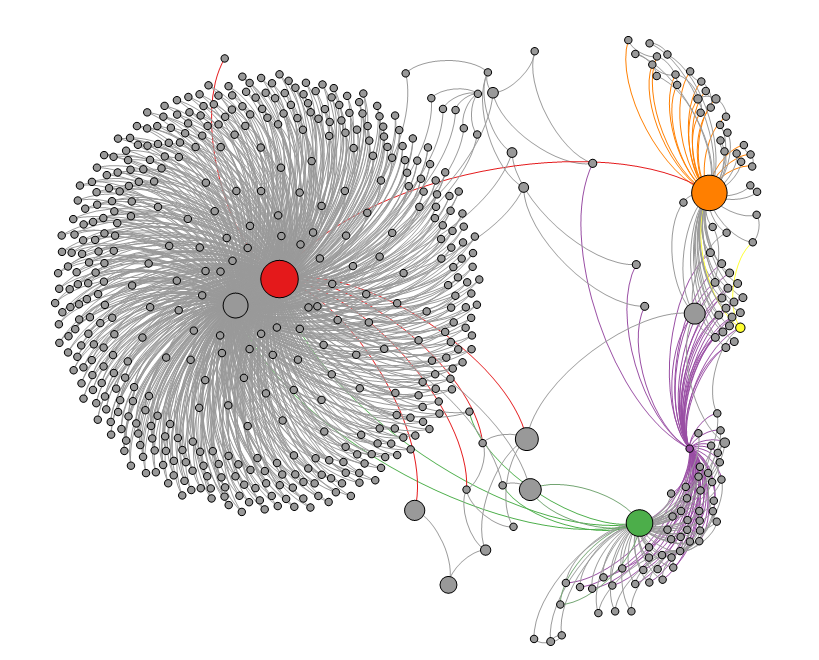
\includegraphics{anonimato_1_11.PNG}
\caption{Visualizzazione egocentrica del ladro nella rete ausiliaria. Gli archi sono colorati in base al vertice sorgente e la dimensione dei vertici è funzione della loro centralità nella rete.\label{anonimato_1_11}}
\end{figure}

Guardando tale rete, si nota come ladro e vittima siano collegati a meno del verso da vertici diversi da quello rappresentante il furto. Ad esempio la figura \ref{anonimato_1_12} evidenzia una sottorete ciclica ricavata dalla rete egocentrica in cui tutti i vertici/indirizzi sono stati contratti in vertici/utente.
Si può notare che il furto delle 25000 BTC è stato preceduto da un piccolo furto di 1 BTC. Inoltre, sfruttando dati off-network, è stato possibile identificare alcuni degli altri utenti coinvolti: il nodo viola è l'account principale della mining pool Slush e il nodo arancione è il computer appartenente al gruppo hacker noto come LulzSec\footnote{\url{http://twitter.com/LulzSec/status/76388576832651265}}. Fu fatto anche un tentativo di associare il gruppo hacker al furto tramite la pubblicazione di un comunicato (disponibile in \url{http://pastebin.com/88nGp508}) in cui l'indirizzo $pk_red$ viene indicato come appartenente a LulzSec e utilizzabile per le donazioni al gruppo. Tale tentativo è un falso in quanto il comunicato successivo alla data del furto.
Dalla rete si vede comunque come il ladro abbia inviato 0.31337 BTC a LulzSec poco dopo il furto, ma non è possibile associarlo ulteriormente con il gruppo.
L'account Slush ha inviato alla vittima un totale di 441.83 BTC in 70 giorni e 0.2 BTC al vertice giallo in un periodo di 2 giorni. Un giorno prima del furto, tale nodo giallo ha effettuato una donazione di 0.120607 BTC a LulzSec. L'utente proprietario del nodo giallo risulta essere proprietario di almeno 5 indirizzi \footnote{\url{http://blockchain.info/it/address/1MUpbAY7rjWxvLtUwLkARViqSdzypMgVW4}\\ \url{http://blockchain.info/it/address/13tst9ukW294Q7f6zRJr3VmLq6zp1C68EK}\\ \url{http://blockchain.info/it/address/1DcQvXMD87MaYcFZqHzDZyH3sAv8R5hMZe}\\ \url{http://blockchain.info/it/address/1AEW9ToWWwKoLFYSsLkPqDyHeS2feDVsVZ}\\ \url{http://blockchain.info/it/address/1EWASKF9DLUCgEFqfgrNaHzp3q4oEgjTsF}} e, come la vittima, è un membro del mining pool Slush e ha donato una volta sola a LulzSec: la sua donazione, il giorno prima del furto, è l'ultima attiva nota di questi indirizzi.

\begin{figure}[htbp]
\centering
%TODO fig 1.12 anonimato
%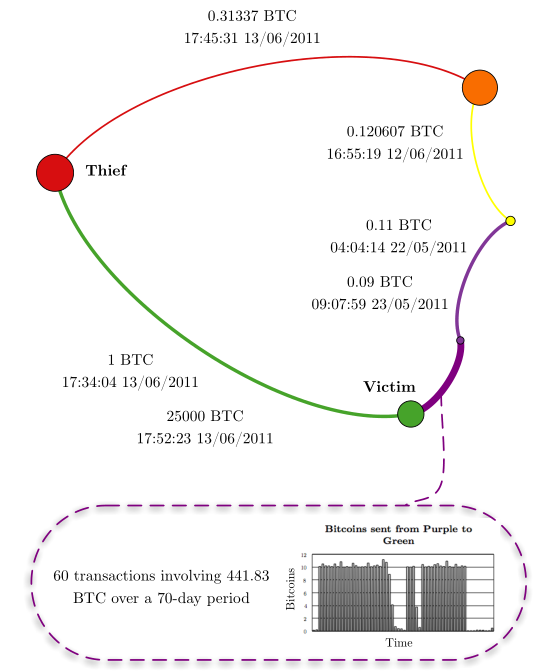
\includegraphics{anonimato_1_12.PNG}
\caption{Ciclo di transazioni che coinvolge ladro, vittima e altri nodi.\label{anonimato_1_12}}
\end{figure}

Dato il grande numero di BTC coinvolte, Harrigan e Reid hanno costruito uno strumento che, dato un vertice di partenza, è in grado tracciare flussi consistenti di BTC nel tempo.
Applicando tale strumento al furto, è stato creato un elenco di indirizzi che hanno ricevuto alcune delle BTC rubate\footnote{elenco completo disponibile nel post del forum che denuncia il furto e in \url{http://folk.uio.no/vegardno/allinvain-addresses.txt}.} contenente più di 34100 voci, inoltre è stato possibile individuare una serie di transazioni interessanti.
Prima tra tutte è il piccolo furto di 1 BTC che ha preceduto di pochissimo il "colpo grosso" da 25000 BTC, in secondo luogo la spartizione di tale somma tra un ristretto numero di indirizzi che poi hanno nuovamente confluito il tutto all'indirizzo di partenza.
A questa fase di smistamento delle BTC sono seguite quattro interessanti transazioni alle 19:49, 20:01, 20:13 e 20:55, le ultime due delle quali sono particolarmente notevoli in quanto passanti tra un gran numero di indirizzi nel giro di poche ore.
Identifichiamo il flusso delle 20:55 come 1 e quello delle 20:13 come 2. Il flusso 1 si divide al vertica A alle 04:05 del giorno dopo il furto, e alcune delle BTC si uniscono al flusso 2 nel vertice B, creando il nuovo flusso 3. Le restanti BTC del flusso 1 passano attraverso numerosi nodi nel corso dei due giorni successivi, creando il flusso 4.
Il 16 Giungo 2011 alle 13.37 un piccolo ammontare di BTC passa dal flusso 3 ad un indirizzo mai visto prima $pk_1$\footnote{\url{http://blockchain.info/it/address/1FKFiCYJSFqxT3zkZntHjfU47SvAzauZXN}}. Circa sette minuti più tardi, un altro piccolo numero di BTC viene trasferito dal flusso 3 ad un altro indirizzo $pk_2$\footnote{\url{http://blockchain.info/it/address/1FhYawPhWDvkZCJVBrDfQoo2qC3EuKtb94}} mai apparso prima. Infine ci sono due transazioni simultanee dal flusso 4 ad altri due nuovi indirizzi $pk_3$\footnote{\url{http://blockchain.info/it/address/1MJZZmmSrQZ9NzeQt3hYP76oFC5dWAf2nD}} e $pk_4$\footnote{\url{http://blockchain.info/it/address/12dJo17jcR78Uk1Ak5wfgyXtciU62MzcEc}}. Questi quattro indirizzi vengono tutti compressi nello stesso utente $C$ nella user network. Una rappresentazione di queste transazioni è visibile nella figura \ref{anonimato_1_13}

\begin{figure}[htbp]
\centering
%TODO fig 1.13 anonimato
%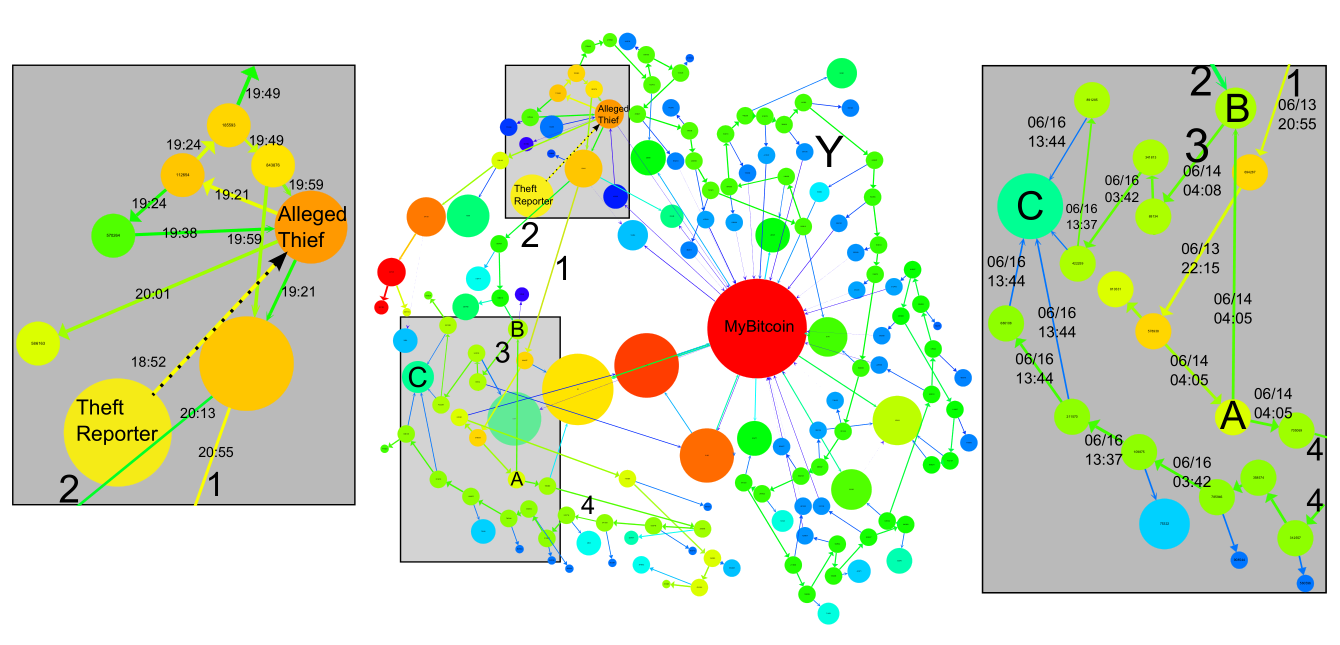
\includegraphics{anonimato_1_13.PNG}
\caption{Flussi di transazioni interessati avvenuti in seguito al furto.\label{anonimato_1_13}}
\end{figure}

Esistono altri flussi interessanti. Ad esempio quello segnato com $Y$ involve il movimento di BTC attraverso 30 indirizzi mai visti prima in un periodo di tempo molto breve. Ad ogni transazione circa 30 BTC (con un valore di mercato di 500\$ ai tempi) vengono risucchiati dal flusso. Il 20 Giugno 2011 alle 12:35 ognuno di questi indirizzi effettua una transazione ad un indirizzo controllato dal servizio MyBitcoin\footnote{\url{http://blockchain.info/it/address/1MAazCWMydsQB5ynYXqSGQDjNQMN3HFmEu}} la quale, coincidenza vuole, era stata precedentemente coinvola in un altro furto\footnote{\url{http://forum.bitcoin.org/index.php?topic=20427.0}}. Questo flusso è visibile in figura \ref{anonimato_1_14}

\begin{figure}[htbp]
\centering
%TODO fig 1.14 anonimato
%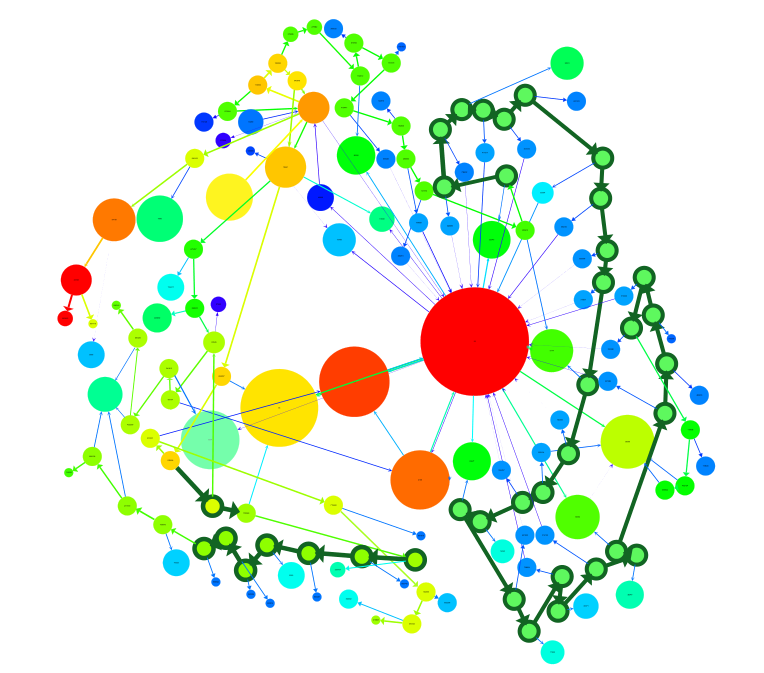
\includegraphics{anonimato_1_14.PNG}
\caption{Transazioni molto rapide in seguito al furto.\label{anonimato_1_14}}
\end{figure}

Tutte queste analisi sono circostanziali. Non è possibile stabilire con certezza se questi flussi implicano una stretta correlazione con i furti, ma sicuramente mettono in luce la quantità di informazioni reperibili e implicano la possibilità che un qualche servizio centrale della rete Bitcoin ne sappia parecchio di più di queste e di altre transazioni.

\section{Contromisure e consigli per aumentare la privacy}

\paragraph{Evitare l'euristica per le transazioni multi-input}

Purtroppo non è possibile evitare facilmente questa euristica senza compromettere le operazioni base della rete Bitcoin.
Infatti la combinazione di molteplici input permette la creazione di valori più grandi da valori più piccoli: se così non fosse ogni transazione dovrebbe avere un valore minore o uguale ai suoi input, fino a quando non raggiunge il valore minimo di 1 Satoshi. In tale situazione, l'unico modo per combinare gli output di più transazioni sarebbe inviare più transazioni separate formate da un singolo input. Questo oltre ad essere decisamente poco pratico non risolve nemmeno il problema dell'euristica, dato che le transazioni possono comunque essere tracciate da $\adversary$ come provenienti dallo stesso portafogli in quanto molto ravvicinate nel tempo.
Un'alternativa potrebbe essere modificare il protocollo in modo da permettere a diversi utenti di partecipare ad una stessa transazione: mentre questa soluzione potrebbe effettivamente ridurre drasticamente l'efficacia dell'euristica, pare improbabile che queste transazioni multi-utente possano avere terreno fertile in Bitcoin.

\paragraph{Evitare l'euristica degli indirizzi ombra}

Mentre evitare la prima euristica è bene o male fattibile, evitare l'utilizzo degli indirizzi ombra è addirittura controproducente in termini di privacy. Senza l'utilizzo di indirizzi ombra infatti, il resto di una transazione verrebbe semplicemente rimesso nell'indirizzo di partenza della transazione stessa, rendendo ancora più facile tracciarne il percorso.
Così come stanno le cose però, sfruttare gli indirizzi ombra causa la dispersione delle monete in diversi indirizzi appartenenti ad uno stesso utente, il che comporta un aggravarsi della falla sfruttabile dall'euristica multi-input.
Una possibile alternativa agli indirizzi ombra consiste in un intervento manuale dell'utente: per prima cosa suddividere le proprie BTC nella quantità necessaria per la transazione e poi effettuare la transazione con resto nullo in un momento successivo, abbastanza distante dal momento di suddivisione per non destare l'attenzione degli algoritmi di clustering.
Una soluzione che comporta la modifica del protocollo, analogamente a quella proposta in precedenza per le transazioni multi-input, consiste nell'implementazione delle transazioni multi-input multi-output, che renderebbero più complesso distinguere un indirizzo ombra da un indirizzo alla sua prima transazione appartenente ad un altro utente.

\paragraph{Implicazioni per l'utilizzo generico di Bitcoin}

Gli autori di \cite{user-privacy}, nonostante la specificità della loro simulazione, ritengono che i risultati trovati possano essere applicati anche ad un utilizzo generico della rete Bitcoin.
Nello specifico, ritengono che $\adversary$ possa estrarre dalla blockchain una piccola porzione di indirizzi che corrispondono ad utenti collocati geograficamente vicino allo stesso $\adversary$, permettendogli quindi di lanciare gli algoritmi di clustering visti in scenari simili a quelli del simulatore.
Ad esempio, se Bitcoin fosse diffuso tra i negozianti (alcuni passi in questa direzione si sono fatti negli ultimi mesi in Brazile, Canada e Nord America), allora $\adversary$ potrebbe estrarre tutti gli indirizzi che interagiscono con i negozianti presenti in una particolare area geografica: più grande il numero di indirizzi di commercianti (fisici) conosciuti, più completa la visione che $\adversary$ ha della rete Bitcoin in quell'area, in quanto si ritiene che solo i clienti più attivi di tali commercianti siano i residenti dell'area.
L'unica soluzione a ciò è rappresentata dall'utilizzo di servizi Bitcoin di terze parti, come banche Bitcoin e anonimizzatori, che nascondano la relazione tra gli input e gli output di una transazione. Ovviamente questa soluzione fa letteralmente a pugni con uno dei motivi principali per cui è stata creata la rete Bitcoin, ovvero la rimozione completa delle ``terze parti'' nelle transazioni. Inoltre si tratta di una relativa \emph{scelta dell'orco}: bisogna rischiare che un $\adversary$ tracci il mio profilo oppure devo fidarmi e lasciare in gestione le mie transazioni\footnote{con relativi BTC miei e delle mie controparti} ad una società che intercede per me, magari anche dietro pagamento?

